\chapter{Evaluation} 
In the project, there were 2 aspects to evaluate- the TML and the website. Both aspects were evaluated continually through unit tests during production.

After the website had been completed, a user evaluation was conducted on second year computing students. TMs are taught after to students that have few years of programming experience, and for this reason second years were chosen. Note that they had little familiarity, if any, with Turing Machines and were introduced to both TMs and TML during the evaluation session. The aim of the evaluation was to:
\begin{itemize}
    \item compare TMs and TML programs;
    \item understand whether students believe writing a TML program would help them in drawing a TM; and
    \item evaluate the structure of the website.
\end{itemize}
The evaluation session also served as a great opportunity to ask for any more features to be added to the website and the language.

During the evaluation session, students were first introduced to the concept of TML, and expected to understand what language two mystery programs accept. Then, they were introduced to TMs, and expected to do the same thing. Finally, they were asked to write some programs in the TML. Some of the difficult programs to write were optional, although many attempted them. The evaluation took about 50 minutes to be completed. The students were asked to fill out a worksheet. They were expected to use the website throughout the session. This helped them get more familiar with the language and TMs, and allowed them to test their own programs for correctness. It also allowed for the evaluation of both the website and the language. After they had completed the worksheet, they completed a survey to evaluate the language and the website. Both the worksheet and the survey are given in the appendix.

\section{Evaluation Results}



% Unit tests all pass. 

% User testing results given by section.

\subsection{Language Evaluation}
The language was continually tested during production to ensure correctness. This was achieved using unit testing. They were used to test all aspects of the parser, and were extensive. In fact, the unit tests had more than $95\%$ code coverage in each part.

During user evaluation, users were asked to evaluate the langugage in the following criteria:
\begin{enumerate}
    \item TML is easy to understand
    \item TML is easy to write programs in
    \item I was able to fix errors in my code using the error messages provided
    \item I was able to easily reason executing a program on a tape
\end{enumerate}
They were asked to rate how much they agreed with each statement, and the result is summarised for each criterion in the violin plot below:
\begin{figure}[H]
    \centering
    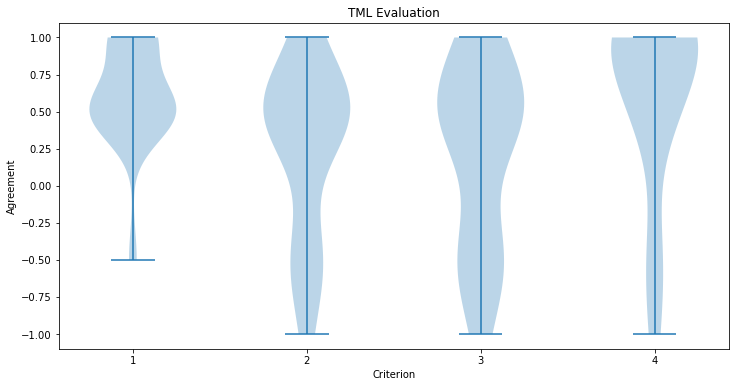
\includegraphics[scale=0.75]{data/tml-evaluation.png}
    \caption{A violin plot that summarises the results of the survey relating to the TML. All the criteria are listed above. The agreement value refers to how much the user agrees to the statement- $-1$ is strongly disagree; $-0.5$ disagree; $0.5$ agree and $1$ strongly agree.}
\end{figure}
\noindent It is clear that most students found the language easy to understand. In particular, the comments in the survey showed that the students found the language intuitive. However, when complex programs were being executed, some students were struggling to follow the code and reason its execution. Similarly, some also found it difficult to write complex programs, such as $a^n b^n c^n$, or understand why it is not as easy as some of the other programs they had encountered before, in particular $a^n b^n$. Nonetheless, many found the error messages quite useful and it helped them write correct programs. 

The TML was then directly compared to TMs. That is, students were asked to compare TMs and TML programs in the following criteria:
\begin{enumerate}
    \item I am more confident in writing a program in TML than drawing a TM
    \item I find it easier to reason what a TML program accepts than a TM
\end{enumerate}
The students were asked to rate how much they agreed with each statement, and the result is summarised for each criterion in the violin plot below:
\begin{figure}[H]
    \centering
    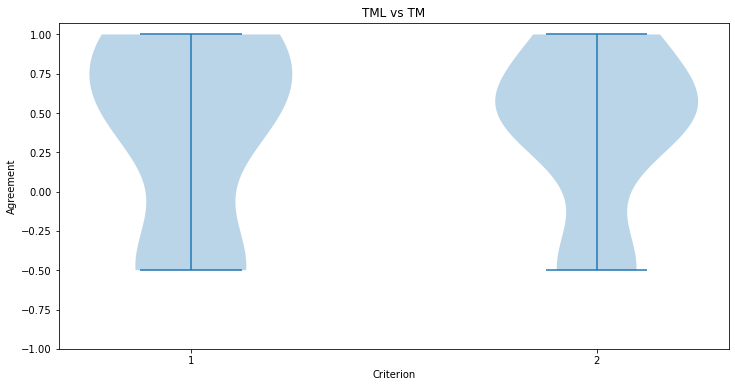
\includegraphics[scale=0.75]{data/tml-v-tm.png}
    \caption{A violin plot that summarises the results of the survey that compare TM and TML.}
\end{figure}
\noindent The results here are more interesting. Overall, students are more confident with TML than TM. This is somewhat expected since the worksheet focuses much more on TML, and students were not asked to draw a TM. Nonetheless, it is clear that the students agree to a lesser extent that it is easier to reason a TML program than a TM. This is quite expected, and I believe they would have found it easier to reason how a TM executes than a TML program since diagrams are easier to follow than code in general. 

The students were then asked whether they would consider writing a TML program before drawing a TM.
\begin{figure}[H]
    \centering
    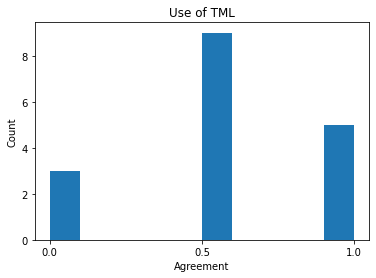
\includegraphics[scale=0.75]{data/use-tml.png}
    \caption{A histogram that summarises whether the users would consider writing a TML program before drawing a TM. 0 means no; 0.5 means maybe; and 1 means yes.}
\end{figure}
\noindent When drawing a TM, it is quite helpful to plan the machine beforehand. TML provides an intermediate opportunity where it is possible to reason in quite a low-level how to execute on a tape, but still keeping it a programming language which makes it easy to write. The results clearly show that many would consider drawing it. The hesitation might result from the little experience that they had gotten; I would imagine that they would benefit writing a TML program especially before drawing some complex TMs.

\subsection{Website Evaluation}

\begin{enumerate}
    \item The website is easy to follow
    \item The presentation of the website is intuitive
    \item There were no visible bugs in the website
    \item The website was fast
    \item The website feels complete
    \item The code execution was easy to follow
    \item The code editor was easy to use
\end{enumerate}

\begin{figure}[H]
    \centering
    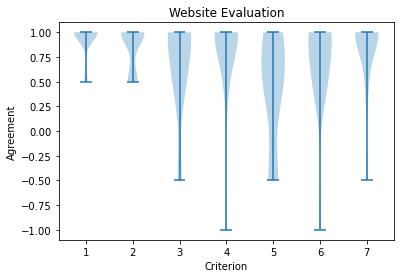
\includegraphics[scale=0.75]{data/website-evaluation.png}
    \caption{A violin plot that summarises the results of the survey relating to the website.}
\end{figure}


% How good is your solution? How well did you solve the general problem, and what evidence do you have to support that?

% \section{Guidance}
% \begin{itemize}
%     \item
%         Ask specific questions that address the general problem.
%     \item
%         Answer them with precise evidence (graphs, numbers, statistical
%         analysis, qualitative analysis).
%     \item
%         Be fair and be scientific.
%     \item
%         The key thing is to show that you know how to evaluate your work, not
%         that your work is the most amazing product ever.
% \end{itemize}

% \section{Evidence}
% Make sure you present your evidence well. Use appropriate visualisations, 
% reporting techniques and statistical analysis, as appropriate. The point is not
% to dump all the data you have but to present an argument well supported by evidence gathered.

% If you use numerical evidence, specify reasonable numbers of significant digits; don't state ``18.41141\% of users were successful'' if you only had 20 users. If you average \textit{anything}, present both a measure of central tendency (e.g. mean, median) \textit{and} a measure of spread (e.g. standard deviation, min/max, interquartile range).

% You can use \texttt{siunitx} to define units, space numbers neatly, and set the precision for the whole LaTeX document. 

% % setup siunitx to have two decimal places
% \sisetup{
% 	round-mode = places,
% 	round-precision = 2
% }

% For example, these numbers will appear with two decimal places: \num{3.141592}, \num{2.71828}, and this one will appear with reasonable spacing \num{1000000}.



% If you use statistical procedures, make sure you understand the process you are using,
% and that you check the required assumptions hold in your case. 

% If you visualise, follow the basic rules, as illustrated in Figure \ref{fig:boxplot}:
% \begin{itemize}
% \item Label everything correctly (axis, title, units).
% \item Caption thoroughly.
% \item Reference in text.
% \item \textbf{Include appropriate display of uncertainty (e.g. error bars, Box plot)}
% \item Minimize clutter.
% \end{itemize}

% See the file \texttt{guide\_to\_visualising.pdf} for further information and guidance.

% \begin{figure}[htb]
%     \centering
%     \includegraphics[width=1.0\linewidth]{images/boxplot_finger_distance.pdf}    

%     \caption{Average number of fingers detected by the touch sensor at different heights above the surface, averaged over all gestures. Dashed lines indicate
%     the true number of fingers present. The Box plots include bootstrapped uncertainty notches for the median. It is clear that the device is biased toward 
%     undercounting fingers, particularly at higher $z$ distances.
%     }

%     % use the notation fig:name to cross reference a figure
%     \label{fig:boxplot} 
% \end{figure}


\section{Evaluation Limitations}

